\section{Механические колебания}
%Сив557
\AddProb Построить графики зависимости от времени смещения, скорости и ускорения при простом гармоническом колебании. Построить графики зависимости скорости и ускорения от смещения. Найти соотношения между амплитудами смещения, скорости и ускорения.

\begin{wrapfigure}[6]{R}{2.3cm}
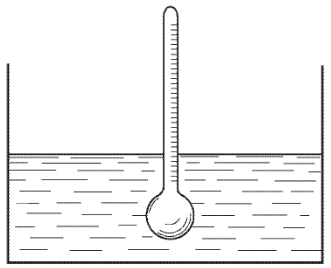
\includegraphics[width=0.2\textwidth]{areometr.png}
\caption{}
\label{areometr}
\end{wrapfigure}
%Сив560
\AddProb Ареометр с цилиндрической трубкой диаметра $D$ (рис. \ref{areometr}), плавающий в жидкости плотности $\rho$, получает небольшой вертикальный толчок. Найти период колебаний $T$ ареометра, если масса его $m$ известна. Движение жидкости и ее сопротивление движению ареометра не учитывать.

\begin{wrapfigure}[8]{R}{3cm}
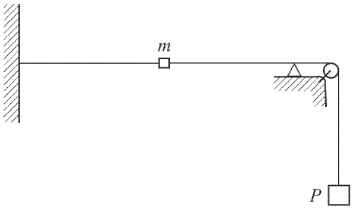
\includegraphics[width=0.3\textwidth]{oscilString.png}
\caption{}
\label{oscilString}
\end{wrapfigure}
%Сив572
\AddProb Найти период свободных малых колебаний грузика массы $m$,
укрепленного на середине тонкой струны длины $L$ (рис. \ref{oscilString}). Массой струны можно пренебречь; натяжение струны постоянно и равно $P$.
%Сив580
\AddProb Горизонтальная мембрана совершает синусоидальные колебания с круговой частотой $\omega$ и и амплитудой $A$. На мембране лежит маленький грузик. При каком условии грузик будет колебаться вместе с мембраной и при каком он начнет подскакивать?

\begin{wrapfigure}[11]{R}{2cm}
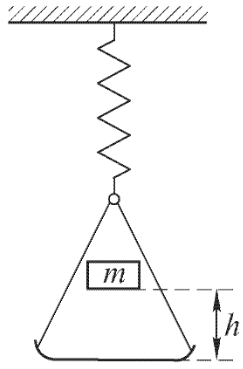
\includegraphics[width=0.2\textwidth]{fallingOnPlate.png}
\caption{}
\label{fallingOnPlate}
\end{wrapfigure}
%Сив582
\AddProb На чашку весов, подвешенную на пружине, падает с высоты $h$ груз массы $m$ и остается на чашке (рис. \ref{fallingOnPlate}), не подпрыгивая относительно нее. Чашка начинает колебаться. Коэффициент жесткости пружины $k$. Определить амплитуду $A$ колебаний (массой чашки и пружины по сравнению с массой груза можно пренебречь).
%Сив558
\AddProb Найти выражения для потенциальной, кинетической и полной энергии материальной точки массы $m$, совершающей гармоническое колебание по закону $A \cos \omega t$.
%Сив565
\AddProb Представьте себе шахту, пронизывающую земной шар по одному из его диаметров. Найти закон движения тела, упавшего в эту
шахту, учитывая изменения значения ускорения свободного падения
внутри Земли. Трение о стенки шахты и сопротивление воздуха не
учитывать.

\begin{wrapfigure}[10]{R}{2cm}
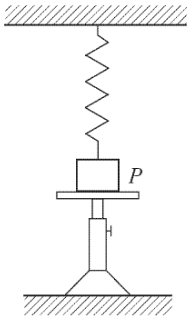
\includegraphics[width=0.2\textwidth]{removePlate.png}
\caption{}
\label{removePlate}
\end{wrapfigure}
%Сив575
\AddProb К пружине, один конец которой закреплен, подвешен груз $P$ массы $m$, лежащий на подставке так, что пружина не растянута (рис. \ref{removePlate}). Без толчка подставка убирается. Найти движение груза и максимальное натяжение пружины. Коэффициент жесткости пружины $k$.
%Сив577
\AddProb На доске лежит груз весом $Р = 10$ Н. Доска совершает гармоническое колебание в вертикальном направлении с периодом $T = 1/2$ с и амплитудой $A = 2$ см. Определить величину силы давления $F$ груза на доску. С какой амплитудой А должна колебаться доска, чтобы груз начал отскакивать от доски?
%Сив581
\AddProb Доска совершает гармоническое колебание в горизонтальном
направлении с периодом $T = 5$ с. Лежащее на ней тело начинает скользить, когда амплитуда колебания достигает величины $A = 0,6$ м. Каков коэффициент трения покоя к между грузом и доской?
\clearpage